\documentclass{beamer}
% \usepackage[brazil]{babel}
\usepackage[utf8]{inputenc}
\usepackage{MnSymbol,wasysym}

\usepackage{fancybox}
\title[\color{white}The Art of Presenting Science]{\Huge The Art of Presenting Science}
%\subtitle[short version]{}
\date[\color{white}October 24, 2019]{October 24, 2019}
\author[\color{white}Sivaram Ambikasaran]{Sivaram Ambikasaran}
% \institute[\color{white}IITM]{IITM}
\usetheme{Madrid}
\newcommand{\BS}[1]{\Huge{Bullshit rule: #1}\\}
\newcommand{\RR}[1]{\color{white}\Huge{Reality rule: #1}\\}
\newcommand{\BBS}{Bullshit Rules}
\newcommand{\RRS}{\color{white}Reality Rules}

 
\usecolortheme{owl}
\setbeamercolor{normal text}{fg=orange}
\usebeamercolor*{normal text}
\setbeamerfont{frametitle}{size=\Huge}

\begin{document}
\frame{\titlepage}

\begin{frame}{\color{white}Greatest communicators}
	\begin{center}
		\color{white}\Huge{Who?}
	\end{center}
\end{frame}

\begin{frame}{\BBS}
	\begin{center}
		\BS{1}
		\Huge{Work will speak for itself}
	\end{center}
\end{frame}

\begin{frame}
	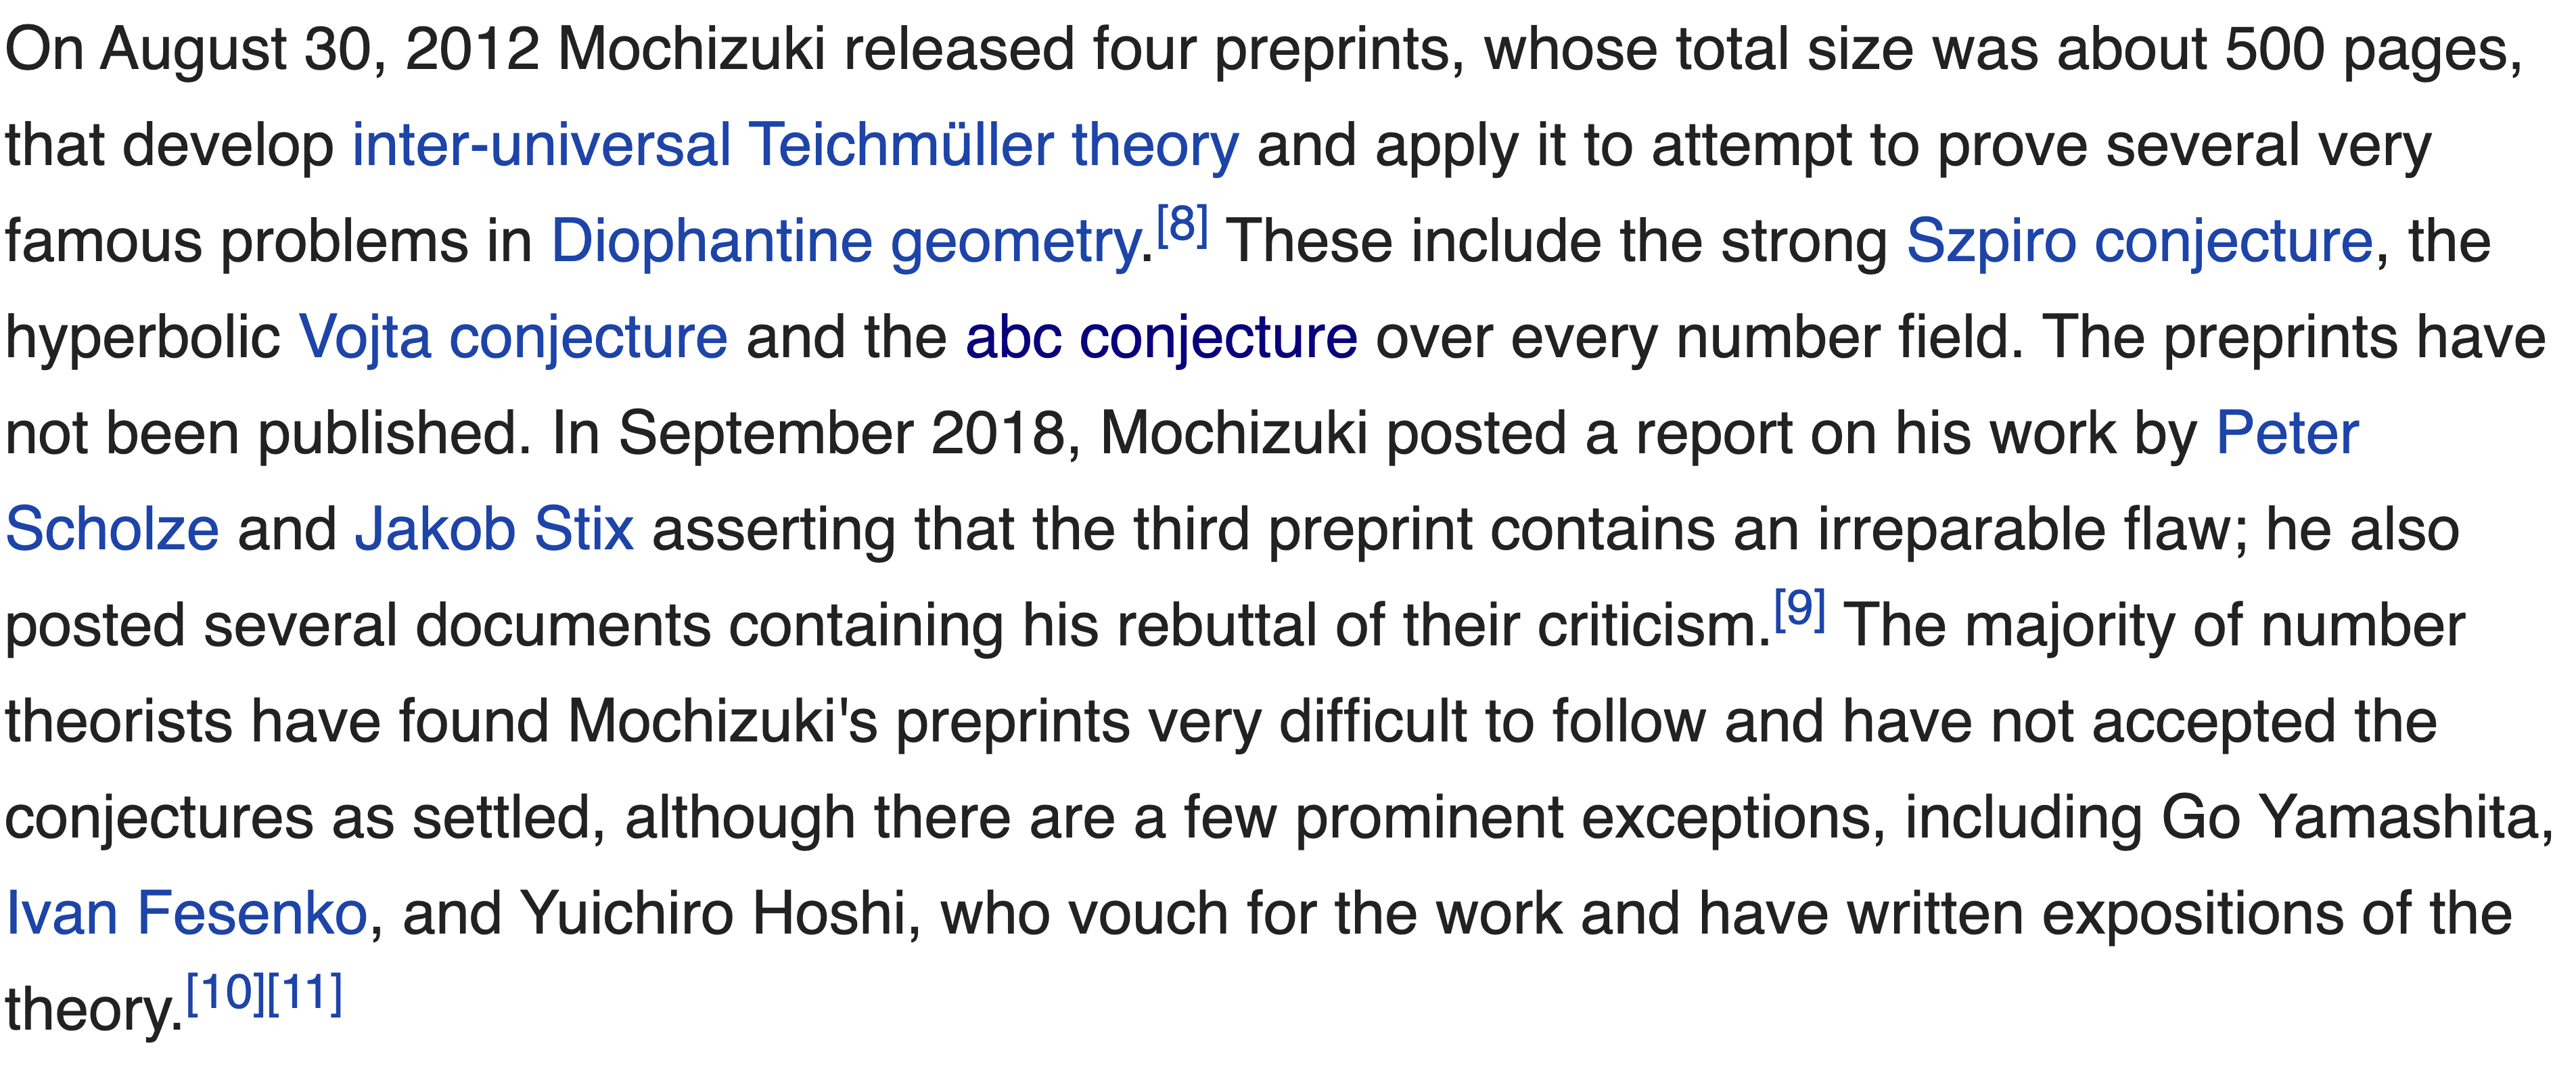
\includegraphics[width=\textwidth]{./Mochizuki.png}
\end{frame}

\begin{frame}{\RRS}
	\begin{center}
		\RR{1}
		\Huge{Your work: your product}\\
		\Huge{Talk: advertisement of your work}\\
		\LARGE{Good product with bad advertisement \frownie{}}\\
		\LARGE{Bad product with good advertisement \frownie{}}\\
	\end{center}
\end{frame}

\begin{frame}{\BBS}
	\begin{center}
		\BS{2}
		\Huge{Every slide must be packed from top left to bottom right with text}
	\end{center}
\end{frame}

\begin{frame}
	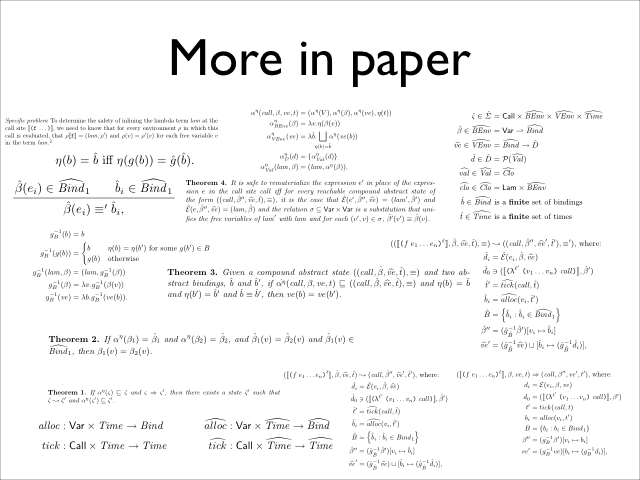
\includegraphics[width=\textwidth]{./garbage.png}
\end{frame}

\begin{frame}{\RRS}
	\begin{center}
		\RR{2}
		\Huge{Minimal text; Each slide should showcase only one thing}\\
		\Huge{\textbf{\emph{YOU}} need to talk about the content}
	\end{center}
\end{frame}

\begin{frame}{\BBS}
	\begin{center}
		\BS{3}
		\Huge{Will convince my audience,\\I have done LOTS of work}
	\end{center}
\end{frame}

\begin{frame}{\RRS}
	\begin{center}
		\RR{3}
		\Huge{Quantity of work doesn't matter}\\
		\Huge{\textbf{Quality} does}
	\end{center}
\end{frame}

\begin{frame}{\BBS}
	\begin{center}
		\BS{4}
		\Huge{Pictures and Figures are pointless}
	\end{center}
\end{frame}

\begin{frame}{\RRS}
	\begin{center}
		\RR{4}
		\Huge{\textbf{Picture is worth a thousand words}}\\
		\Huge{\emph{Even in mathematical communication}}
	\end{center}
\end{frame}

\begin{frame}{\BBS}
	\begin{center}
		\BS{5}
		\Huge{Present every single step in proof so that people will know I have done it correctly}
	\end{center}
\end{frame}

\begin{frame}{\RRS}
	\begin{center}
		\RR{5}
		\Huge{Writing an article is different from presenting your work}\\
		\pause
		\Huge{Encapsulate the ideas of the theorems and proofs}\\
		\pause
		\Huge{True understanding}
	\end{center}
\end{frame}

\begin{frame}{\BBS}
	\begin{center}
		\BS{6}
		\Huge{Don't talk about failures or incorrect attempts}
	\end{center}
\end{frame}

\begin{frame}{\RRS}
	\begin{center}
		\RR{6}
		\Huge{The path you took is more important than result}
	\end{center}
\end{frame}

\begin{frame}{\BBS}
	\begin{center}
		\BS{7}
		\Huge{Be serious;\\No jokes, no deviations;\\Only content}
	\end{center}
\end{frame}

\begin{frame}{\RRS}
	\begin{center}
		\RR{7}
		\Huge{Your audience are not ROBOTS}
	\end{center}
\end{frame}
%
% \begin{frame}{\BBS}
% 	\begin{center}
% 		\BS{8}
% 		\Huge{Voice, body language, excitement, should not be given attention to.}
% 	\end{center}
% \end{frame}

\begin{frame}{\BBS}
	\begin{center}
		\BS{8}
		\Huge{Same content works for all audience}
	\end{center}
\end{frame}

\begin{frame}{\RRS}
	\begin{center}
		\RR{8}
		\Huge{Audience are our customers}
	\end{center}
\end{frame}

\begin{frame}{\BBS}
	\begin{center}
		\BS{9}
		\Huge{No need to motivate the talk}
	\end{center}
\end{frame}

\begin{frame}{\RRS}
	\begin{center}
		\RR{9}
		\Huge{Spend almost a quarter of the talk on motivation}
	\end{center}
\end{frame}

\begin{frame}{\BBS}
	\begin{center}
		\BS{10}
		\Huge{More slides $\implies$ More work}
	\end{center}
\end{frame}

\begin{frame}{\RRS}
	\begin{center}
		\RR{10}
		\Huge{If I Had More Time, I Would Have Written a Shorter Letter.}
	\end{center}
\end{frame}

\begin{frame}{\BBS}
	\begin{center}
		\BS{11}
		\Huge{Talk fast $\implies$ More words $\implies$ More work}
	\end{center}
\end{frame}

\begin{frame}{\RRS}
	\begin{center}
		\RR{11}
		\Huge{Talk short sentences at the right pace.}
	\end{center}
\end{frame}

\begin{frame}{\BBS}
	\begin{center}
		\BS{12}
		\Huge{Presentations should be monologue.}
	\end{center}
\end{frame}


\begin{frame}{\RRS}
	\begin{center}
		\RR{12}
		\Huge{Engage your audience.}
	\end{center}
\end{frame}

\begin{frame}{\color{white}Other points to remember}
	\begin{center}
		\color{white}\Huge{Have a catchy title}
	\end{center}
\end{frame}

\begin{frame}{\color{white}Other points to remember}
	\begin{center}
		\color{white}\Huge{Do not have an outline slide}\\
		\color{white}\Huge{It is boring; Suspense is lost}
	\end{center}
\end{frame}

\begin{frame}{\color{white}Other points to remember}
	\begin{center}
		\color{white}\Huge{Start with a question or an interesting fact}\\
		\pause
		\Huge{Use that as a motivation}
	\end{center}
\end{frame}

\begin{frame}{\color{white}Other points to remember}
	\begin{center}
		\color{white}
		\Huge{Tell a story}\\
		\Huge{Build up the suspense}
	\end{center}
\end{frame}



\begin{frame}{\color{white}Other points to remember}
	\begin{center}
		\color{white}
		\Huge{Do not memorize your talk!}\\
		\pause
		\Huge{Try to adapt on the fly!}\\
		\pause
		\Huge{Extempore!}
	\end{center}
\end{frame}

\begin{frame}{\color{white}Other points to remember}
	\begin{center}
		\color{white}
		\Huge{You are the hero(ine)!}\\
		\pause
		\Huge{Don't become a villain!}
	\end{center}
\end{frame}

\begin{frame}{\color{white}Other points to remember}
	\begin{center}
		\color{white}
		\Huge{Show current slide/total slides}\\
		\pause
		\Huge{Have a good climax}\\
		\pause
		\Huge{Finish on time with a bang!}\\
	\end{center}
\end{frame}
% 	\begin{itemize}
% 		\item
% 		Work will speak for itself
% 		\item
% 		Long boring talks
% 		\item
% 		Catchy title
% 		\item
% 		Start with catchy facts
% 		\item
% 		Talking to human beings and not machines
% 		\item
% 		Have a story to tell
% 		\item
% 		Think of your talk as a movie; How to keep your audience engaged;
% 		Romantic movie, Horror, Thriller
% 		\item
% 		Think of yourself as Shahrukh or Rajni or Amitabh
% 		\item
% 		Pictures
% 		\item
% 		In any communication content plays a small role compared to voice and body language
% 	\end{itemize}
% \end{frame}
%
% \begin{frame}
% 	Despite multiple conferences dedicated to explicating Mochizuki’s proof, number theorists have struggled to come to grips with its underlying ideas. His series of papers, which total more than 500 pages, are written in an impenetrable style, and refer back to a further 500 pages or so of previous work by Mochizuki, creating what one mathematician, Brian Conrad of Stanford University, has called “a sense of infinite regress.”
% \end{frame}
\end{document}